\documentclass[conference]{IEEEtran}
\IEEEoverridecommandlockouts

\usepackage{cite}
\usepackage{amsmath,amssymb,amsfonts}
\usepackage{graphicx}
\usepackage{booktabs}
\usepackage{xcolor}
\usepackage{hyperref}
\usepackage{balance}

\hypersetup{
  colorlinks=true,
  linkcolor=blue!60!black,
  citecolor=blue!60!black,
  urlcolor=blue!60!black
}

\begin{document}

\title{White-Box Composable Skill Graphs with Defect Knowledge Feedback for Safe, Zero-LLM-Replay Web Verification}

\author{
\IEEEauthorblockN{[Author Name]}
\IEEEauthorblockA{\textit{[Department of Computer Science / Software Engineering]} \\
\textit{[University Name]} \\
[City, Country] \\
[author.email@university.edu]}
}

\maketitle

\begin{abstract}
End-to-end (E2E) web verification faces a sharp tension between fragility and cost. Static browser scripts run deterministically at negligible cost but break whenever benign UI labels or layouts evolve, whereas autonomous Large Language Model (LLM) web agents adapt dynamically yet incur high latency, stochastic failures, and recurring token cost on every verification run. Worse, black-box LLM self-healers that lack source-code visibility and telemetry gating risk \emph{false healing}---weakening or deleting test oracles to make real product regressions appear green.

We present a \textbf{White-Box Composable Skill Graph} closed-loop architecture unified with a deterministic \textbf{Defect Knowledge Graph} and exposed to coding agents via a zero-dependency local Model Context Protocol (MCP) server. Atomic UI workflows are authored once with parameterized inputs, statically grounded to source files via AST/URL adapters, and replayed deterministically at \textbf{0 LLM calls}. Upon failure, a telemetry-and-oracle gate strictly separates benign \texttt{SKILL\_DRIFT} (triggering bounded $k \le 2$ scoped \texttt{git diff}-guided self-healing with immutable postconditions) from genuine \texttt{PRODUCT\_BUG} regressions (enforcing a hard \textbf{0-LLM refusal} and emitting schema-validated \texttt{DRAFT} defect records isolated from human-\texttt{CONFIRMED} knowledge).

Evaluated across two contrasting open-source full-stack applications (\texttt{cypress-realworld-app} in React/Express/GraphQL and \texttt{horilla} in Python/Django/HTMX), our system achieves \textbf{25/25 (100\%)} pass rate at \textbf{5.07\,s/run} vs.\ \textbf{11/15 (73.3\%, Fisher $p = 0.015$)} at \textbf{102.34\,s/run} for a fair Pure-LLM baseline (\textbf{20.2$\times$ speedup}, Mann-Whitney $U = 0$, $p < 0.001$, Cliff's $\delta = -1$, \textbf{98.5\%} cost reduction at $N = 100$). On our 48-commit fault-evolution benchmark (\texttt{EvoBench-48}), White-Box achieves \textbf{16/16 (100.0\%)} drift recovery vs.\ \textbf{50.0\%} for Black-Box (Exact McNemar $p = 0.0078$) while eliminating attempted oracle weakening (\textbf{0/20} vs.\ \textbf{12/20}, Fisher $p < 0.001$) and false healing (\textbf{0/20} vs.\ \textbf{1/20} live masked regression). Across three LLM families (\texttt{DeepSeek-V3.2}, \texttt{Gemini-2.5-Flash}, \texttt{GPT-4o-mini}), White-Box maintains \textbf{24/24 (100\%)} drift recovery and \textbf{0/12 (0\%)} false healing at \textbf{0} LLM calls on bugs. Finally, replaying \textbf{99} real upstream Git commits (\texttt{RealGit-99}, 0-LLM) skips \textbf{92.9\%} of commits and achieves \textbf{98.5\%} test reduction at \textbf{0.17--0.21\,ms/commit}.
\end{abstract}

\begin{IEEEkeywords}
End-to-End Web Testing, Self-Healing Tests, Large Language Models, Regression Test Selection, Defect Knowledge Graph, Model Context Protocol.
\end{IEEEkeywords}

\section{Introduction}
Automated end-to-end (E2E) browser testing remains indispensable for catching cross-layer regressions spanning frontend components, HTTP/GraphQL APIs, and database persistence. Yet engineering teams face an uncomfortable dilemma in continuous integration (CI). Traditional Playwright or Cypress suites~\cite{playwright2024} execute rapidly and deterministically without inference cost, but even minor UI refinements---such as renaming a form placeholder or button label---break locators and stall deployment pipelines. Conversely, emerging LLM-driven web agents~\cite{zhou2024webarena,deng2023mind2web,zheng2024seeact} navigate unfamiliar interfaces dynamically, but re-discovering the same multi-step workflow on every commit multiplies latency by an order of magnitude, incurs recurring API expenses, and introduces non-deterministic execution failures.

A popular middle ground is \emph{self-healing test automation}~\cite{choudhary2011water,stocco2018vista}, increasingly augmented with LLMs to repair broken selectors at runtime. However, we observe a critical safety flaw in black-box LLM self-healers: when a failure stems from a genuine \emph{product defect}---such as an HTTP 500 server crash, a swallowed click handler, or a silent HTTP 200 persistence omission---an unguarded LLM healer frequently attempts to \emph{weaken or delete postcondition assertions} in order to satisfy its repair prompt. In our empirical evaluation, black-box healing attempted oracle weakening on 60\% of real product regressions and actively produced live \emph{false heals} that turned genuine regressions into green \texttt{VERIFIED\_PASS} runs across both \texttt{DeepSeek-V3.2} and \texttt{Gemini-2.5-Flash}.

To resolve both the amortization problem and the false-healing hazard simultaneously, we design and evaluate a \textbf{White-Box Composable Skill Graph} closed-loop architecture unified with a deterministic \textbf{Defect Knowledge Graph}. Rather than treating the web application as an opaque DOM tree, our system grounds every atomic, parameterized UI skill directly to its implementing frontend components, backend routes, and templates using zero-LLM static adapters. Verification runs execute deterministically at \textbf{0 LLM calls}, while LLM inference is invoked solely on two rare, tightly gated paths: (i) one-time parameterized skill authoring validated by a mandatory fresh-data replay gate, and (ii) bounded $k \le 2$ white-box repair guided by scoped \texttt{git diff} hunks when---and only when---deterministic telemetry confirms benign UI drift rather than a product defect.

Furthermore, when a genuine \texttt{PRODUCT\_BUG} is detected, the verifier refuses healing at \textbf{0 LLM calls} and automatically emits a schema-validated \texttt{DRAFT} defect record linked to the failing code units and telemetry. A deterministic graph compiler compiles curated invariants, guardrails, and reviewed bugs into a Defect Knowledge Graph while strictly isolating provisional \texttt{DRAFT} observations from human-\texttt{CONFIRMED} truth. Both graphs are exposed to IDE coding agents through a zero-dependency local Model Context Protocol (MCP) server~\cite{mcp2024}, closing the loop from commit diff to risk-prioritized verification and defect memory.

\textbf{Contributions.} This paper makes four concrete contributions:
\begin{enumerate}
  \item \textbf{White-Box Composable Skill Graph \& Telemetry Gate:} A formal skill representation combining precondition DAG planning, static AST/URL route-to-code grounding (React/Express/GraphQL and Django/HTMX), zero-LLM Playwright verification, and a deterministic 3-way fault oracle separating \texttt{VERIFIED\_PASS}, \texttt{SKILL\_DRIFT}, and \texttt{PRODUCT\_BUG}.
  \item \textbf{Safe Bounded Self-Healing \& Generalization-Gated Authoring:} A scoped \texttt{git diff}-guided repair loop ($k \le 2$) enforcing immutable postconditions and hard 0-LLM refusal on product bugs, paired with modal-aware authoring guarded by mandatory unseen-data replay.
  \item \textbf{Closed-Loop Defect Knowledge Unification \& Local MCP Server:} A deterministic knowledge bridge emitting schema-valid \texttt{DRAFT} bugs and \texttt{PROPOSED} guardrails, defect-aware risk prioritization with sibling-defect propagation, and a zero-dependency MCP stdio server (6 tools, 2 resources).
  \item \textbf{Rigorous Dual-Stack \& Multi-Model Evaluation:} Comprehensive empirical evaluation across two contrasting real open-source applications spanning \texttt{RQ1} cost/latency amortization, \texttt{EvoBench-48} (48 deterministic commits with Wilson 95\% CIs, Exact McNemar, and Fisher's Exact tests), a 3-family LLM generalization panel (\texttt{DeepSeek-V3.2}, \texttt{Gemini-2.5-Flash}, \texttt{GPT-4o-mini}), and \texttt{RealGit-99} (99 real upstream Git commits replayed at 0-LLM).
\end{enumerate}

\section{Problem Formulation}
We model a web application under test (SUT) at repository commit $c$ with changed file set $\Delta F(c)$ and unified diff $\Delta D(c)$.

\textbf{Composable Skill Graph.} A Skill Graph is a tuple $G_S = (S, E_{\text{pre}})$, where each atomic skill $s \in S$ is a schema-validated YAML specification:
\begin{equation}
  s = \langle \mathit{id}, P_{\text{in}}, \mathit{Pre}, \mathit{Eff}, A, \Omega, C_{\text{ref}} \rangle
\end{equation}
comprising typed parameter bindings $P_{\text{in}}$, required symbolic state facts $\mathit{Pre}$, produced state effects $\mathit{Eff}$, an ordered sequence of semantic UI actions $A$ (using closed locator strategies \texttt{role}, \texttt{label}, \texttt{placeholder}, \texttt{text}, \texttt{testid}, and \texttt{title}), verifiable postconditions $\Omega$ (DOM visibility/containment/absence, URL transition, and HTTP response status checks), and static source code references $C_{\text{ref}} = \langle F_s, R_s \rangle$ mapping $s$ to source files $F_s$ and API/route paths $R_s$. Given a target verification goal $g$ and actor bindings, a deterministic backward-chaining planner computes a minimal executable DAG plan $\pi = [s_1, \dots, s_m]$ satisfying all preconditions (including multi-actor workflows such as sender--receiver payment approval).

\textbf{Deterministic 3-Way Fault Oracle.} Executing $\pi$ in a clean browser context produces telemetry $\tau = \langle H_{5\text{xx}}, J_{\text{err}}, \sigma_{\text{step}}, \omega_{\text{res}} \rangle$, recording same-origin HTTP $\ge 500$ responses ($H_{5\text{xx}}$), uncaught JavaScript runtime exceptions ($J_{\text{err}}$), step-level semantic locator outcomes ($\sigma_{\text{step}}$), and postcondition receipts ($\omega_{\text{res}}$). The deterministic oracle $\Phi(\tau)$ assigns one of three mutually exclusive verdicts:
\begin{equation}
\Phi(\tau) =
\begin{cases}
  \texttt{PRODUCT\_BUG} & \text{if } |H_{5\text{xx}}| > 0 \lor |J_{\text{err}}| > 0 \lor \exists \omega \in \Omega: \neg \omega \\
  \texttt{SKILL\_DRIFT} & \text{if } |H_{5\text{xx}}| = 0 \land |J_{\text{err}}| = 0 \land \text{locator\_miss}(\sigma_{\text{step}}) \\
  \texttt{VERIFIED\_PASS} & \text{otherwise.}
\end{cases}
\end{equation}
Critically, even if a step fails to locate a control, the presence of a server crash or runtime exception overrides classification to \texttt{PRODUCT\_BUG}, ensuring that crashes hiding UI controls are never misclassified as benign UI drift.

\textbf{Defect Knowledge Graph.} A compiled Defect Knowledge Graph $G_D = (V_D, E_D)$ indexes defect families, domain invariants, executable guardrails (including \texttt{SKILL\_GRAPH\_VERIFIER} guardrails referencing skill IDs), and defect records partitioned strictly by provenance into human-\texttt{CONFIRMED} knowledge $V_D^{\text{conf}}$ and machine-observed provisional records $V_D^{\text{draft}}$.

\section{System Architecture and Methodology}
Fig.~\ref{fig:architecture} illustrates the end-to-end closed-loop workflow spanning five deterministic and bounded-LLM stages.

\begin{figure*}[t]
  \centering
  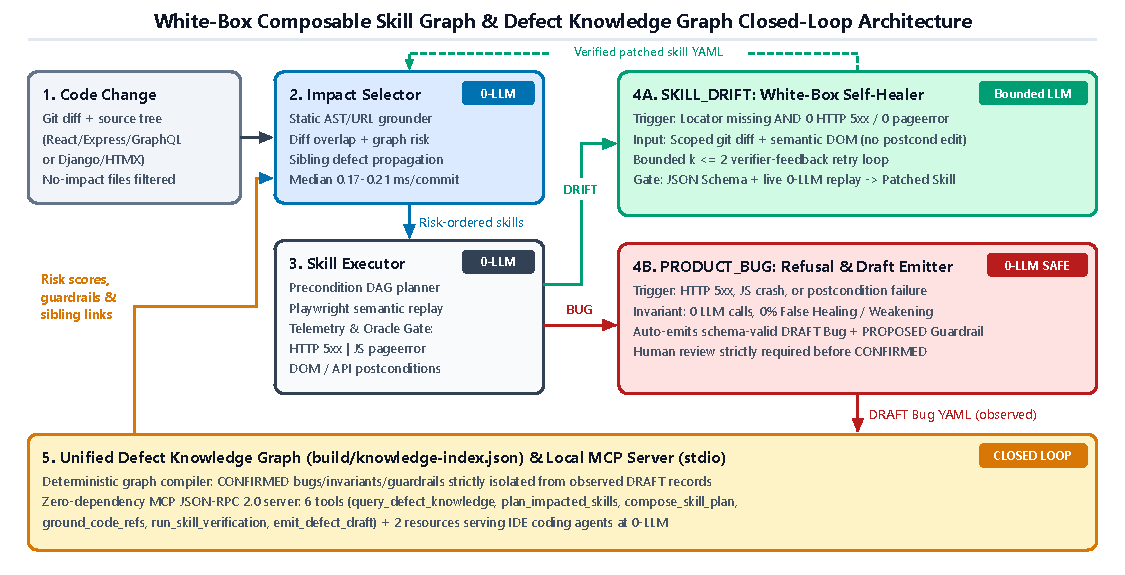
\includegraphics[width=\textwidth]{figures/fig1-architecture.pdf}
  \caption{End-to-end closed-loop architecture uniting the White-Box Composable Skill Graph, deterministic 3-way Telemetry Oracle, bounded $k \le 2$ self-healer, hard 0-LLM product-bug refusal gate, compiled Defect Knowledge Graph, and zero-dependency local MCP server.}
  \label{fig:architecture}
\end{figure*}

\subsection{Static Route-to-Code Grounding (0-LLM)}
Early prototypes often link tests to code via naive keyword search, injecting substantial false-positive files. We replace keyword grep with a plugin-based deterministic static grounder (\texttt{grounder.ts}) operating exclusively on local source trees and observed runtime routes/endpoints at 0-LLM:
\begin{itemize}
  \item \textbf{\texttt{TsWebRouteGrounder}:} Resolves React Router paths to page/container components, traverses 1-hop ES/TS imports to forms/items, matches Express route registrations (\texttt{app.use}, \texttt{router.post/patch/delete}), and maps GraphQL operations to resolver files.
  \item \textbf{\texttt{DjangoRouteGrounder}:} Recursively resolves \texttt{urls.py} and \texttt{include()} trees, maps class-based view \texttt{.as\_view()} symbols, performs 2-hop same-file CBV superclass inheritance traversal to recover shared templates and \texttt{form\_class} Python modules, respects theme-priority template directories, resolves \texttt{?model=app.Model} query parameters, and filters generic HTTP error/permission fallbacks.
\end{itemize}

\subsection{Defect-Aware Impact Selection and Sibling Propagation}
Given commit file changes $\Delta F(c)$, a baseline white-box selector activates skill $s$ iff $F_s \cap \Delta F(c) \neq \emptyset$ and extracts scoped unified diff hunks restricted to $F_s$. Our unified selector (\texttt{defect-aware-impact.ts}) enriches this with $G_D$:
\begin{enumerate}
  \item \textbf{Risk-Score Prioritization:} Skills linked to \texttt{CONFIRMED} defects, violated invariants, or \texttt{ACTIVE} guardrails receive higher risk weights than plain file-overlap skills, executing the highest-risk workflows first.
  \item \textbf{Sibling Defect Propagation:} When $\Delta F(c)$ touches code units linked via \texttt{SIBLING\_CANDIDATE} edges in $G_D$, the selector expands impact to sibling skills guarding unmodified peer code units sharing the same defect family.
  \item \textbf{Provenance Isolation:} Confirmed knowledge signals and observed \texttt{DRAFT} signals are computed and reported in separate fields; provisional drafts can inform ranking but never masquerade as confirmed invariants.
\end{enumerate}

\subsection{Bounded White-Box Self-Healing ($k \le 2$) and Hard Refusal}
When $\Phi(\tau) = \texttt{PRODUCT\_BUG}$, the healer immediately returns \texttt{REFUSED\_PRODUCT\_BUG} with \textbf{0 LLM calls}. Only when $\Phi(\tau) = \texttt{SKILL\_DRIFT}$ does the bounded repair loop execute for up to $k \le 2$ attempts:
\begin{itemize}
  \item \textbf{Attempt 1:} Supplies the LLM with the failing skill YAML, failing step diagnostic, semantic DOM snapshot, and the \emph{scoped \texttt{git diff}} restricted strictly to $F_s$.
  \item \textbf{Structural Immutability Guard:} Before live execution, the candidate patch is validated against \texttt{skill.schema.json} and checked deterministically to verify that all postconditions $\Omega$ are structurally preserved (no deletions or semantic weakening).
  \item \textbf{Attempt 2 (Verifier Feedback):} If Attempt 1 violates schema constraints or fails live clean-DB Playwright replay without triggering HTTP 5xx/\texttt{pageerror}, exact verifier diagnostics are injected into Attempt 2. Any HTTP 5xx or \texttt{pageerror} during replay aborts healing immediately as a hidden \texttt{PRODUCT\_BUG}.
\end{itemize}

\subsection{Modal-Aware Authoring and Generalization Gate}
To author new skills without hand-writing YAML, our explorer (\texttt{author.ts}) observes semantic DOM snapshots where visible active modal controls (\texttt{[MODAL]}, including checkboxes with resolved \texttt{<label for>} and icon-only \texttt{title} attributes) are prioritized ahead of ambient sidebar links, paired with bounded modal/HTMX hydration waits and automatic dismissal of unsolicited onboarding tours. Crucially, every candidate skill must pass a \textbf{mandatory 0-LLM generalization gate}: it is parameterized (replacing concrete sample strings with \texttt{\{\{param\}\}} templates) and replayed on a reset database with completely unseen fresh inputs using \textbf{0 LLM calls}.

\subsection{Closed-Loop Defect Emission and Local MCP Server}
On every \texttt{PRODUCT\_BUG} verdict, \texttt{knowledge-bridge.ts} converts grounded files and failing endpoints into closed POSIX-safe stable \texttt{codeUnitId} keys (\texttt{:ts:}, \texttt{:py:}, \texttt{:template:}, \texttt{:api:}) and emits a schema-valid \texttt{DRAFT} bug YAML (with explicit human-review placeholders so \texttt{knowledge-validator} structurally blocks any automated promotion to \texttt{CONFIRMED}). All capabilities are exposed over a zero-dependency JSON-RPC 2.0 local MCP stdio server (\texttt{packages/mcp-server/}) providing 6 tools (\texttt{query\_defect\_knowledge}, \texttt{plan\_impacted\_skills}, \texttt{compose\_skill\_plan}, \texttt{ground\_code\_refs}, \texttt{run\_skill\_verification}, \texttt{emit\_defect\_draft}) and 2 catalog resources.

\section{Experimental Design}
We evaluate the system across five research questions:
\begin{itemize}
  \item \textbf{RQ1 (Cost \& Latency Amortization):} How do reliability, latency, and cumulative cost compare between 0-LLM Skill Graph replay and a fair Pure-LLM browser agent?
  \item \textbf{RQ2 (Fault Discrimination \& Safe Self-Healing):} On \texttt{EvoBench-48}, how accurately does White-Box recover UI drift while preventing oracle weakening and false healing compared to Static, Black-Box, and Telemetry-Gated No-Diff baselines?
  \item \textbf{RQ3 (Cross-Model Generalization):} Are White-Box recovery and 0\% false-healing safety preserved across contrasting LLM families?
  \item \textbf{RQ4 (Real-World Commit Replay):} What test reduction and selection latency does 0-LLM impact selection achieve on genuine upstream Git history (\texttt{RealGit-99})?
  \item \textbf{RQ5 (Grounding, Authoring \& Closed-Loop Unification):} How much do Phase A static grounding / modal authoring and Phase B defect-aware MCP unification improve precision, authoring success, top-1 risk accuracy, and sibling recall?
\end{itemize}

\textbf{Target Open-Source Systems.} All experiments run live against unmodified upstream checkouts of two contrasting full-stack web applications without Docker: (1) \texttt{cypress-io/cypress-realworld-app} (TypeScript, React 18, MUI, XState, Express, GraphQL, \texttt{lowdb}; 8 skills) and (2) \texttt{horilla-opensource/horilla} (Python 3.12, Django 5.2, HTMX, SQLite; 4 skills). Databases are reset cleanly before every timed trial and repository working trees are restored to \texttt{HEAD} after every mutation.

\textbf{Benchmarks and Controls.}
\begin{itemize}
  \item \textbf{\texttt{EvoBench-48}:} 48 deterministic mutations across both stacks comprising 16 \texttt{SKILL\_DRIFT} commits (label, placeholder, button, and form field evolutions across TSX, Django templates, and Python \texttt{forms.py}), 20 \texttt{PRODUCT\_BUG} commits (HTTP 500 crashes, GraphQL mutation errors, swallowed UI handlers, silent HTTP 200 DB omissions, broken filters/auth), and 12 \texttt{NO\_IMPACT} commits.
  \item \textbf{\texttt{RealGit-99}:} 99 consecutive real upstream Git commit pairs (49 on \texttt{cypress-rwa}, 50 on \texttt{horilla}) replayed strictly read-only at 0-LLM.
  \item \textbf{3-Model Panel:} Apples-to-apples live evaluation of \texttt{deepseek/deepseek-v3.2}, \texttt{google/gemini-2.5-flash}, and \texttt{openai/gpt-4o-mini} ($T = 0$, JSON mode) on 8 shared drifts, 4 representative product bugs, and 2 cross-stack authoring tasks.
  \item \textbf{Fairness:} All baselines (Pure-LLM Agent, Black-Box Healer, Telemetry-Gated No-Diff Healer) share the exact same LLM client, semantic DOM snapshotter, Playwright executor, and postcondition verifier.
\end{itemize}

\textbf{Statistical Methodology.} Proportions are reported with exact Wilson score 95\% confidence intervals~\cite{wilson1927}. Paired binary healing comparisons on identical \texttt{EvoBench-48} commits use exact two-sided McNemar tests~\cite{mcnemar1947}; unpaired contingency tables (pass rate, weakening, FHR) use exact two-sided Fisher's exact tests~\cite{fisher1922}; non-parametric latency distributions use two-sided Mann-Whitney $U$ tests~\cite{mann1947} paired with Cliff's $\delta$ effect sizes~\cite{cliff1993,romano2006}.

\section{Evaluation Results}

\subsection{RQ1: Cost and Latency Amortization}
Across 5 multi-step workflows (including a 2-user, 5-skill payment-request approval chain on \texttt{cypress-rwa} and a 3-skill login--create--search chain on \texttt{horilla}), Table~\ref{tab:rq1-amortization} and Fig.~\ref{fig:rq1} summarize measured and projected performance. Skill Graph achieved \textbf{25/25 (100.0\%, CI [86.7, 100.0])} \texttt{VERIFIED\_PASS} at a median of \textbf{4.47\,s} (mean 5.07\,s, 0 LLM calls), whereas the Pure-LLM baseline achieved \textbf{11/15 (73.3\%, CI [48.0, 89.1])} at a median of \textbf{113.25\,s} (mean 102.34\,s, 14.4 LLM calls/run). Both gains are statistically significant: Fisher's exact $p = 0.015$ for pass rate, and Mann-Whitney $U = 0$, $p < 0.001$ with maximum effect size Cliff's $\delta = -1.0$ (large) for execution latency (\textbf{20.2$\times$ speedup}). Amortizing one-time authoring cost (\$0.00322) plus a 4\% periodic drift rate (1 white-box heal every 25 runs) yields \textbf{88.17\%} cost savings at $N = 5$ measured cycles and \textbf{98.52\%} at $N = 100$ cycles (\$0.00807 vs.\ \$0.54430).

\begin{table*}[t]
\centering
\caption{RQ1: Cost and Latency Amortization Across Repeated Verification Cycles (DeepSeek-V3.2)}
\label{tab:rq1-amortization}
\begin{tabular}{rlrrrrrrr}
\toprule
$N$ & Basis & Pure Calls & Pure Cost (\$) & Pure Time (s) & SG Calls & SG Cost (\$) & SG Time (s) & Savings (\%) \\
\midrule
1 & Measured & 14.4 & \$0.00544 & 102.3 & 7 & \$0.00322 & 5.1 & 40.81\% \\
5 & Measured & 72 & \$0.02722 & 511.7 & 7 & \$0.00322 & 25.4 & 88.17\% \\
10 & Projected & 144 & \$0.05443 & 1023.4 & 7 & \$0.00322 & 50.7 & 94.08\% \\
25 & Projected & 360 & \$0.13608 & 2558.6 & 8 & \$0.00443 & 126.9 & 96.74\% \\
50 & Projected & 720 & \$0.27215 & 5117.2 & 9 & \$0.00564 & 253.7 & 97.93\% \\
100 & Projected & 1440 & \$0.54430 & 10234.3 & 11 & \$0.00807 & 507.4 & 98.52\% \\
\bottomrule
\end{tabular}
\\[4pt]
\footnotesize{Pass rate: Skill Graph 25/25 (100.0\% [86.7, 100.0]) vs.\ Pure-LLM 11/15 (73.3\% [48.0, 89.1]), Fisher $p = 0.015$. Latency: median 4.47\,s vs.\ 113.25\,s, MW $U = 0$, $p < 0.001$, Cliff's $\delta = -1$ (large).}
\end{table*}

\begin{figure*}[t]
  \centering
  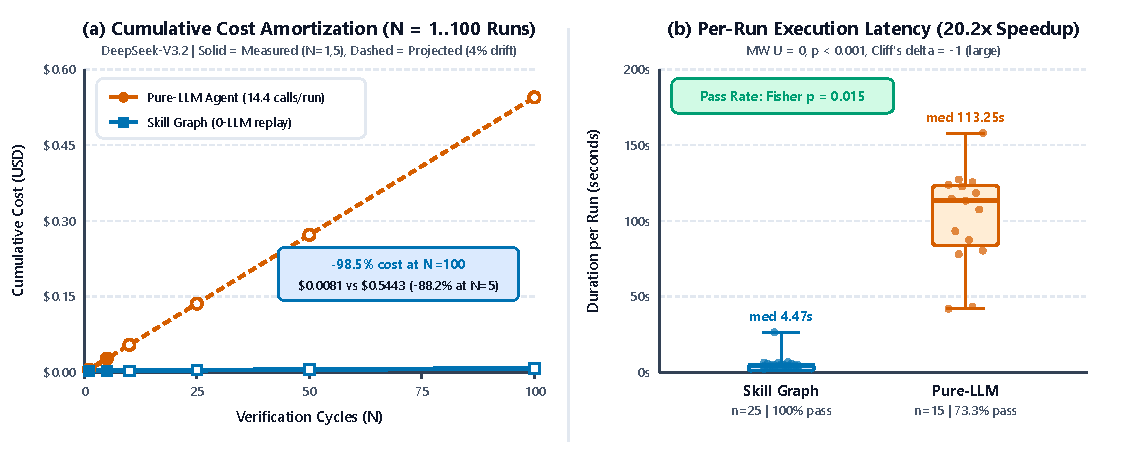
\includegraphics[width=\textwidth]{figures/fig2-rq1-amortization.pdf}
  \caption{RQ1 evaluation: (a) cumulative cost amortization from $N = 1$ to $100$ runs showing 88.2\% measured savings at $N = 5$ and 98.5\% at $N = 100$; (b) per-run execution latency distributions demonstrating a 20.2$\times$ mean speedup ($U = 0, p < 0.001, \delta = -1$).}
  \label{fig:rq1}
\end{figure*}

\subsection{RQ2: Fault Discrimination and Safe Healing on \texttt{EvoBench-48}}
Table~\ref{tab:evobench48-stats} and Fig.~\ref{fig:evobench48} report complete ablation results across all 48 commits. Deterministic fault classification and white-box impact selection both achieved \textbf{48/48 (100.0\%)} exact accuracy with \textbf{80.74\%} test reduction (57/296 skill executions).

On the 16 \texttt{SKILL\_DRIFT} commits, Drift Recovery Rate (DRR) improves monotonically across ablations: Static \textbf{0.0\%} (0/16) $\rightarrow$ Black-Box \textbf{50.0\%} (8/16, CI [28.0, 72.0]) $\rightarrow$ Telemetry-Gated No-Diff \textbf{81.3\%} (13/16, CI [57.0, 93.4]) $\rightarrow$ \textbf{White-Box Skill Graph ($k \le 2$) 100.0\%} (16/16, CI [80.6, 100.0]). Paired Exact McNemar confirms statistical significance over Static ($b = 16, c = 0, p < 0.001$) and Black-Box ($b = 8, c = 0, p = 0.0078$). Notably, on server-side Django form/template drifts (\texttt{HOR-D2}, \texttt{HOR-D3}, and \texttt{HOR-D4} in Python \texttt{base/forms.py}), only the scoped \texttt{git diff}-guided White-Box healer succeeded while both Black-Box and No-Diff failed ($b = 3, c = 0, p = 0.250$ vs.\ No-Diff).

On the 20 \texttt{PRODUCT\_BUG} commits, the safety contrast is stark: Black-Box wasted 36 LLM calls (2.25$\times$ White-Box), attempted to weaken or delete postconditions on \textbf{12/20 (60.0\%, CI [38.7, 78.1])} real bugs, and committed a live \textbf{False Heal (5.0\%, 1/20)} on \texttt{RWA-B8} (silently dropping transaction persistence while marking the suite \texttt{VERIFIED\_PASS}). By contrast, White-Box refused all 20 bugs at \textbf{0 LLM calls}, achieving \textbf{0.0\% (0/20, CI [0.0, 16.1])} Attempted Weakening (Fisher $p < 0.001$) and \textbf{100.0\% (20/20)} Bug Detection.

\begin{table*}[t]
\centering
\caption{EvoBench-48 ($N=48$: 16 Drift, 20 Product Bug, 12 No-Impact) System Comparison with Wilson 95\% Confidence Intervals and Significance Tests}
\label{tab:evobench48-stats}
\begin{tabular}{lrrrrrr}
\toprule
System & DRR (95\% Wilson CI) & Att.\ Weakening (95\% CI) & FHR (95\% CI) & Bug Det. & Calls & Est.\ USD \\
\midrule
Static Playwright (0-LLM) & 0.0\% [0.0, 19.4] & 0.0\% & 0.0\% & 100.0\% & 0 & \$0.0000 \\
Black-Box Healer (No Diff/Gate) & 50.0\% [28.0, 72.0] & 60.0\% [38.7, 78.1] & 5.0\% [0.9, 23.6] & 95.0\% & 36 & \$0.0432 \\
Telemetry-Gated (No Diff) & 81.3\% [57.0, 93.4] & 0.0\% [0.0, 16.1] & 0.0\% [0.0, 16.1] & 100.0\% & 17 & \$0.0198 \\
\textbf{White-Box Skill Graph ($k \le 2$)} & \textbf{100.0\% [80.6, 100.0]} & \textbf{0.0\% [0.0, 16.1]} & \textbf{0.0\% [0.0, 16.1]} & \textbf{100.0\%} & \textbf{16} & \textbf{\$0.0191} \\
\bottomrule
\end{tabular}
\\[4pt]
\footnotesize{Exact McNemar DRR $p$-values (White-Box vs.\ Static: $p < 0.001$; vs.\ Black-Box: $p = 0.0078$; vs.\ No-Diff: $p = 0.250$). Fisher's Exact Safety $p$-value (Attempted Weakening vs.\ Black-Box): $p < 0.001$. Impact Selection: 48/48 exact match, 80.74\% test reduction.}
\end{table*}

\begin{figure*}[t]
  \centering
  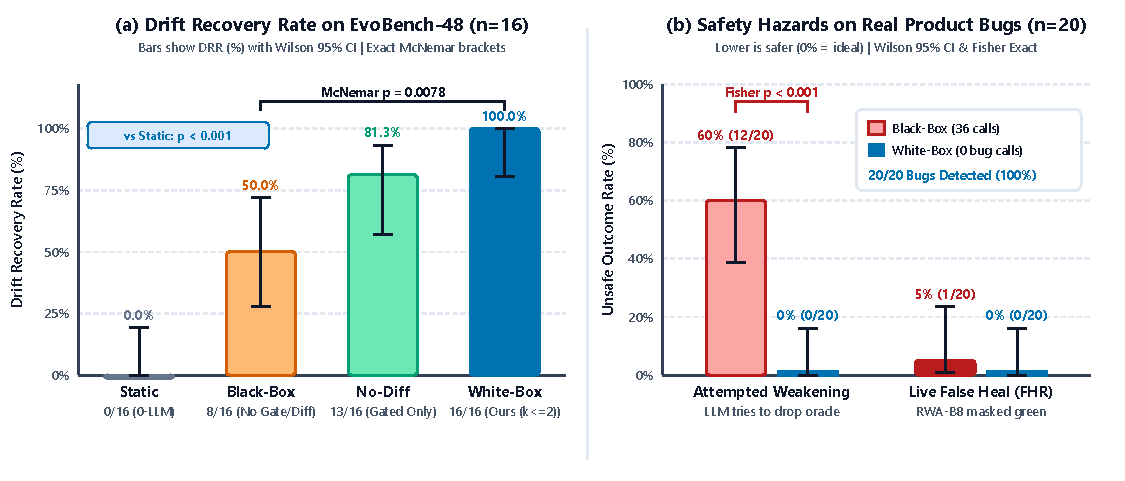
\includegraphics[width=\textwidth]{figures/fig3-evobench48-ablation.pdf}
  \caption{EvoBench-48 ablation results: (a) Drift Recovery Rate across four system variants with Wilson 95\% confidence intervals and Exact McNemar brackets; (b) Safety hazards on 20 real product regressions demonstrating elimination of oracle weakening ($p < 0.001$) and false healing.}
  \label{fig:evobench48}
\end{figure*}

\subsection{RQ3: Cross-Model Generalization Across 3 LLM Families}
Table~\ref{tab:multimodel} and Fig.~\ref{fig:multimodel} confirm that our architecture generalizes across open-weights (\texttt{DeepSeek-V3.2}), Google (\texttt{Gemini-2.5-Flash}), and OpenAI (\texttt{GPT-4o-mini}) model families. Every model achieved \textbf{8/8 (100.0\%)} White-Box DRR---including \texttt{Gemini-2.5-Flash} recovering \texttt{RWA-D5} on Attempt 2 via our bounded $k \le 2$ verifier-feedback loop---and \textbf{0/4 (0\%)} False Healing at \textbf{0 LLM calls} on product bugs (combined \textbf{24/24} DRR and \textbf{0/12} FHR). By contrast, Black-Box healing was inconsistent (50.0\%--87.5\% DRR), wasted 12 calls per model, attempted weakening on \texttt{GPT-4o-mini} (\texttt{HOR-B2}), and caused a live \textbf{False Heal on \texttt{Gemini-2.5-Flash}} (masking real HTTP 500 bug \texttt{RWA-B6} as green). Total White-Box heal cost across all 8 drifts ranged from just \textbf{\$0.0038} (\texttt{GPT-4o-mini}) to \textbf{\$0.0212} (\texttt{Gemini-2.5-Flash}). On cross-stack authoring, \texttt{DeepSeek-V3.2} and \texttt{GPT-4o-mini} passed \textbf{2/2}, while \texttt{Gemini-2.5-Flash} passed \textbf{1/2} (authoring Django \texttt{work\_type.create} in only 5 calls).

\begin{table*}[t]
\centering
\caption{RQ3: Cross-Model Generalization Across 3 LLM Families (8 Shared Drifts, 4 Product Bugs, 2 Cross-Stack Authoring Tasks)}
\label{tab:multimodel}
\begin{tabular}{lrrrrrrr}
\toprule
LLM Model Family & WB DRR & BB DRR & WB Bug Calls / FHR & BB Weakening / FHR & Authoring & WB Calls (USD) & BB Calls (USD) \\
\midrule
DeepSeek-V3.2 & 8/8 (100.0\%) & 4/8 (50.0\%) & 0 / 0/4 (0\%) & 0/4 / 0/4 & 2/2 & 8 (\$0.0099) & 12 (\$0.0146) \\
Gemini-2.5-Flash & 8/8 (100.0\%) & 7/8 (87.5\%) & 0 / 0/4 (0\%) & 1/4 / 1/4 & 1/2 & 9 (\$0.0212) & 12 (\$0.0285) \\
GPT-4o-mini & 8/8 (100.0\%) & 6/8 (75.0\%) & 0 / 0/4 (0\%) & 1/4 / 0/4 & 2/2 & 8 (\$0.0038) & 12 (\$0.0050) \\
\bottomrule
\end{tabular}
\end{table*}

\begin{figure*}[t]
  \centering
  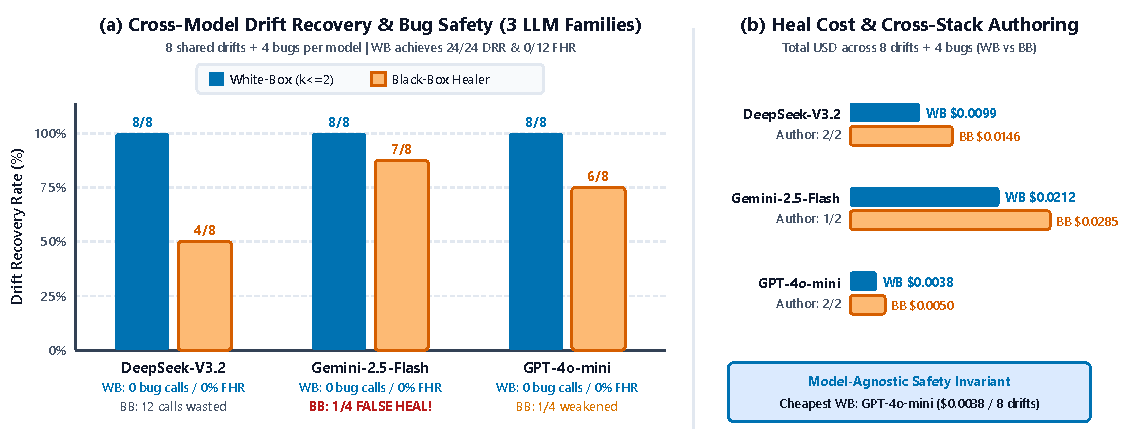
\includegraphics[width=\textwidth]{figures/fig4-multimodel-panel.pdf}
  \caption{Cross-model evaluation across three distinct LLM families: (a) White-Box achieves 100\% DRR (24/24) and 0\% FHR (0/12) across all families whereas Black-Box exhibits live false healing on Gemini-2.5-Flash; (b) per-model healing cost and cross-stack authoring rates.}
  \label{fig:multimodel}
\end{figure*}

\subsection{RQ4: Real-World Upstream Git Commit Replay (\texttt{RealGit-99})}
To validate ecological realism beyond synthetic mutations, Table~\ref{tab:realgit} and Fig.~\ref{fig:realgit}(a) report read-only 0-LLM impact selection across \textbf{99 consecutive real upstream Git commits}. On \texttt{cypress-rwa} (49 commits), 48/49 (98.0\%) required zero E2E executions, achieving \textbf{99.7\%} test reduction at \textbf{0.21\,ms} median latency (P95 0.39\,ms), while accurately activating the grounded skill when ESLint/GraphQL commit \texttt{3aab985} modified \texttt{Query.ts}. On \texttt{horilla} (50 commits), 44/50 (88.0\%) were skipped, achieving \textbf{96.0\%} test reduction at \textbf{0.17\,ms} median latency (P95 0.33\,ms), while activating relevant auth/form skills on real commits touching \texttt{login.html}, \texttt{base/views.py} (\texttt{6a9053e}), and \texttt{generic/form.html} (\texttt{80bea6f}). Combined across both repositories, \textbf{92/99 (92.9\%)} real commits were skipped with \textbf{98.5\%} overall test reduction.

\begin{table}[t]
\centering
\caption{RQ4: Real-World Upstream Git Commit Replay (RealGit-99, 0-LLM)}
\label{tab:realgit}
\begin{tabular}{lrrrrr}
\toprule
Repository & Commits & Skip \% & Reduct.\ \% & Med.\ (ms) & P95 (ms) \\
\midrule
\texttt{cypress-rwa} & 49 & 98.0\% & 99.7\% & 0.21 & 0.39 \\
\texttt{horilla} & 50 & 88.0\% & 96.0\% & 0.17 & 0.33 \\
\midrule
\textbf{Combined} & \textbf{99} & \textbf{92.9\%} & \textbf{98.5\%} & --- & --- \\
\bottomrule
\end{tabular}
\end{table}

\subsection{RQ5: Static Grounding, Authoring Gate, and Unified Graph MCP Loop}
Table~\ref{tab:phase-ab} and Fig.~\ref{fig:realgit}(b) quantify the architectural upgrades across Phases A and B:
\begin{itemize}
  \item \textbf{Static Route-to-Code Grounding:} Replacing keyword grep with \texttt{TsWebRouteGrounder} and \texttt{DjangoRouteGrounder} increased \texttt{codeRefs} micro-average precision from \textbf{25.0\% (6/24)} to \textbf{81.0\% (17/21)}, eliminating noisy cross-app false files (e.g., \texttt{user.settings\_update}: 16.7\% $\rightarrow$ 100.0\%; \texttt{department.delete}: 0.0\% $\rightarrow$ 83.3\%).
  \item \textbf{Modal-Aware Authoring \& Generalization Gate:} Authoring succeeded on \textbf{4/4 (100.0\%)} cross-stack workflows including Horilla's 3-checkbox protected modal \texttt{department.delete} (up from 3/4), while disabling the generalization gate caused \textbf{0/4 (0\%)} fresh-data passes---proving every authored skill would otherwise overfit sample inputs.
  \item \textbf{Unified Defect-Aware Impact \& Live MCP Loop (0-LLM):} Integrating compiled Defect Knowledge Graph risk scores and \texttt{SIBLING\_CANDIDATE} edges improved Top-1 Risk Accuracy from \textbf{2/4 (50.0\%)} to \textbf{4/4 (100.0\%)} and Sibling Regression Recall from \textbf{0/2 (0.0\%)} to \textbf{2/2 (100.0\%)} while keeping 100\% \texttt{NO\_IMPACT} precision. End-to-end child-process MCP stdio verification succeeded on both stacks (\texttt{RWA-B1} and \texttt{HOR-B1}) at \textbf{\$0.00} cost, emitting schema-valid \texttt{DRAFT} bugs (\texttt{BUG:cypress-rwa:170917871}, \texttt{BUG:horilla:58040835}), raising subsequent skill risk scores (+5), and maintaining strict isolation from \texttt{CONFIRMED} knowledge.
\end{itemize}

\begin{table}[t]
\centering
\caption{RQ5: Phase A \& Phase B Engineering Gains (Before vs.\ After)}
\label{tab:phase-ab}
\begin{tabular}{lrr}
\toprule
Evaluation Metric & Baseline & Upgraded (Ours) \\
\midrule
Static \texttt{codeRefs} Precision (0-LLM) & 25.0\% (6/24) & \textbf{81.0\% (17/21)} \\
Cross-Stack Authoring (4 workflows) & 75.0\% (3/4) & \textbf{100.0\% (4/4)} \\
Top-1 Defect Risk Accuracy (0-LLM) & 50.0\% (2/4) & \textbf{100.0\% (4/4)} \\
Sibling Regression Recall (0-LLM) & 0.0\% (0/2) & \textbf{100.0\% (2/2)} \\
Live MCP Closed Loop (0-LLM) & N/A & \textbf{2/2 PASS (\$0.00)} \\
\bottomrule
\end{tabular}
\end{table}

\begin{figure*}[t]
  \centering
  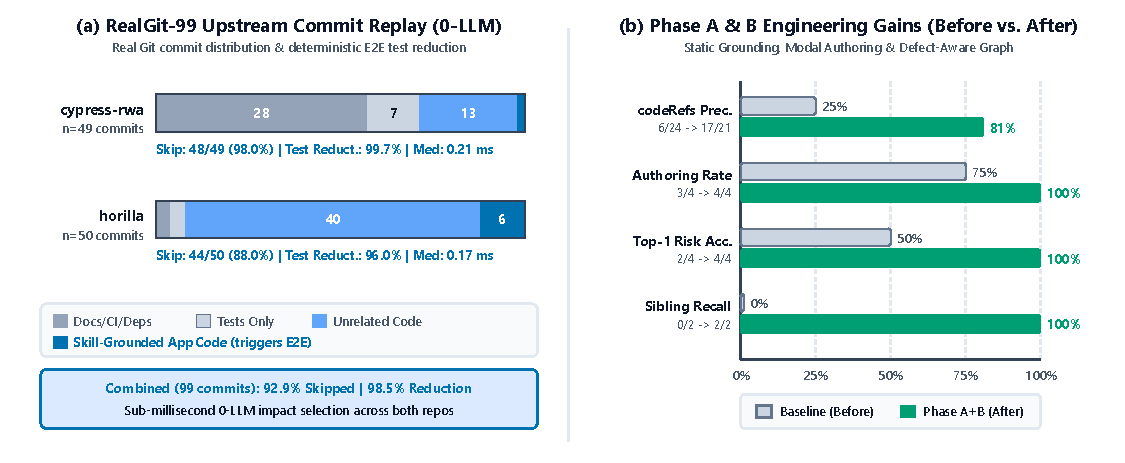
\includegraphics[width=\textwidth]{figures/fig5-realgit-and-grounding.pdf}
  \caption{Ecological validity and engineering gains: (a) RealGit-99 read-only replay across 99 real upstream commits achieving 98.5\% test reduction in sub-millisecond time; (b) Phase A static grounding / modal authoring and Phase B unified graph gains.}
  \label{fig:realgit}
\end{figure*}

\section{Discussion and Threats to Validity}
We highlight five concrete threats to validity and design trade-offs transparently:
\begin{enumerate}
  \item \textbf{Statistical Power of \texttt{git diff} Delta ($p = 0.250$):} While White-Box outperformed Telemetry-Gated No-Diff by $+18.7$ percentage points (16/16 vs.\ 13/16, winning 3--0 on server-side Django form/template drifts with zero losses), $n = 16$ drifts is underpowered for two-sided Exact McNemar significance at $\alpha = 0.05$. Expanding server-side drift suites is planned future work.
  \item \textbf{Skill Coverage Bound on \texttt{RealGit-99}:} Our repositories currently model 8 skills on \texttt{cypress-rwa} and 4 core workflows on \texttt{horilla}. Because \texttt{horilla} contains additional unmodeled modules (e.g., Payroll, Recruitment), 98.5\% test reduction represents an upper bound relative to current skill coverage, though filtering of CI, dependency, documentation, and test-only commits generalizes independently of suite size.
  \item \textbf{Framework Adapter Extensibility:} Static grounding currently ships adapters for React/Express/GraphQL and Django/HTMX. Supporting additional stacks (e.g., Angular/Spring Boot or Next.js App Router) requires authoring a lightweight plugin adapter ($\approx$150--250 LOC per framework). Changes strictly outside tracked source files (pure CSS tweaks, environment flags, external DB migrations) are outside file-overlap scope.
  \item \textbf{Conservative Oracle Trade-Off:} Our telemetry oracle intentionally favors bug safety over aggressive self-healing. Purely aesthetic layout regressions without postconditions are not detected; conversely, an intentional product copy change altering text verified inside a postcondition is conservatively flagged as \texttt{PRODUCT\_BUG} for human review rather than silently auto-patched.
  \item \textbf{Cross-Model Authoring Variance:} Although bounded healing achieved 100\% across all three LLM families, open-ended multi-step authoring still reflects model planning capability (\texttt{DeepSeek-V3.2} and \texttt{GPT-4o-mini}: 2/2; \texttt{Gemini-2.5-Flash}: 1/2).
\end{enumerate}

\section{Related Work}
\textbf{Self-Healing Web Testing.} Classical repair approaches such as WATER~\cite{choudhary2011water} and VISTA~\cite{stocco2018vista} rely on DOM attribute similarity or computer-vision matching across consecutive versions. Unlike purely black-box DOM/visual repairers, our architecture incorporates scoped white-box \texttt{git diff} hunks and enforces a deterministic telemetry gate that structurally prohibits weakening postconditions during product regressions.

\textbf{Autonomous LLM Web Agents.} Benchmarks such as WebArena~\cite{zhou2024webarena}, Mind2Web~\cite{deng2023mind2web}, and grounded agents like SeeAct~\cite{zheng2024seeact} evaluate general-purpose zero-shot web navigation. Our work targets the complementary continuous verification setting: compiling repeatable workflows into deterministic 0-LLM skills amortizes inference cost by 98.5\% and accelerates execution by 20.2$\times$ while retaining LLM adaptability strictly for authoring and drift recovery.

\textbf{Regression Test Selection (RTS).} File- and dependency-level RTS systems such as Ekstazi~\cite{gligoric2015ekstazi} and STARTS~\cite{legunsen2017starts} accelerate unit test suites via bytecode/class dependencies. We bring white-box RTS to full-stack E2E browser skills across JavaScript/TypeScript and Python/Django, further augmenting selection with Defect Knowledge Graph risk scores, active guardrails, and sibling-defect propagation over MCP~\cite{mcp2024}.

\section{Conclusion and Future Work}
We presented a White-Box Composable Skill Graph unified with a deterministic Defect Knowledge Graph and exposed over a local MCP server. Across two contrasting open-source stacks, 48 controlled fault-evolution commits, 99 real upstream Git commits, and three distinct LLM families, our system demonstrates that decoupling 0-LLM deterministic verification from tightly gated, diff-guided self-healing simultaneously delivers 20.2$\times$ faster execution, 98.5\% cost amortization, 100\% drift recovery, and a model-agnostic 0\% false-healing safety guarantee. Future work will extend static grounder plugins to Angular and Spring Boot enterprise stacks, integrate dynamic coverage traces for config-driven routes, and evaluate continuous learning on multi-hundred-skill industrial repositories.

\balance
\bibliographystyle{IEEEtran}
\bibliography{references}

\end{document}
